%% Adaptado de 
%% http://www.ctan.org/tex-archive/macros/latex/contrib/IEEEtran/
%% Traduzido para o congresso de IC da USP
%%*****************************************************************************
% Não modificar

\documentclass[twoside,conference,a4paper]{IEEEtran}

%******************************************************************************
% Não modificar
\usepackage{IEEEtsup} % Definições complementares e modificações.
\usepackage[utf8]{inputenc} % Disponibiliza acentos.
\usepackage[english,brazil]{babel}
%% Disponibiliza Inglês e Português do Brasil.
\usepackage{latexsym,amsfonts,amssymb} % Disponibiliza fontes adicionais.
\usepackage{theorem} 
\usepackage[cmex10]{amsmath} % Pacote matemático básico 
\usepackage{url} 
%\usepackage[portuges,brazil,english]{babel}
\usepackage{graphicx}
\usepackage{amsmath}
\usepackage{amssymb}
\usepackage{color}
\usepackage[pagebackref=true,breaklinks=true,colorlinks,bookmarks=false]{hyperref}
\hypersetup{
    colorlinks=true,
    linkcolor=cyan,
}
\usepackage[tight,footnotesize]{subfigure} 
\usepackage[noadjust]{cite} % Disponibiliza melhorias em citações.
%%*****************************************************************************

\begin{document}
\selectlanguage{brazil}
\renewcommand{\IEEEkeywordsname}{Palavras-chave}

%%*****************************************************************************

\urlstyle{tt}
% Indicar o nome do autor e o curso/nível (grad-mestrado-doutorado-especial)
\title{Identificação de Tweets Sobre Desastres}
\author{%
 \IEEEauthorblockN{Eduardo Barros Innarelli\,\IEEEauthorrefmark{1}}
 \IEEEauthorblockA{\IEEEauthorrefmark{1}%
                   Ciência da Computação - Graduação \\
                   E-mail: e170161@dac.unicamp.br}
 \and
 \IEEEauthorblockN{Victor Ferreira Ferrari\,\IEEEauthorrefmark{2}}
 \IEEEauthorblockA{\IEEEauthorrefmark{2}%
                   Engenharia de Computação - Graduação \\
                   E-mail: v187890@dac.unicamp.br}
 \and
 \IEEEauthorblockN{Vinicius Couto Espindola\,\IEEEauthorrefmark{3}}
 \IEEEauthorblockA{\IEEEauthorrefmark{3}%
                   Engenharia de Computação - Graduação \\
                   E-mail: v188115@dac.unicamp.br}
}

%%*****************************************************************************

\maketitle

%%*****************************************************************************
% Resumo do trabalho
\begin{abstract}
 
 O trabalho é focado na classificação textual de mensagens de redes sociais (tuítes) para identificação de relatos de acidentes, ferramenta que seria aplicável à segurança pública. Para lidar com o problema foram testadas diversas técnicas de aprendizado supervisionado, desde simples, como Regressão Logística, passando por Redes Convolucionais e Recorrentes, até modelos complexos e mais recentes, como BERT. BERT superou todos os concorrentes, com seu próprio pré-processamento e codificação da entrada. Foram obtidos resultados de 83,04\% de acurácia no conjunto de treinamento, 84,12\% de acurácia no conjunto de validação, e 83,02\% de acurácia no conjunto de teste. No entanto, modelos extremamente simples aparentaram obter resultados próximos ao BERT em muito menos tempo. 
 
 
%  Descrever brevemente o problema no qual você está trabalhando: 
%    - Por que você está desenvolvendo este trabalho? 
%    - Qual a motivação para este desenvolvimento?
%    - Por que ele é importante? 
%  Descritivo da metodologia: 
%    - Que problema foi tratado? 
%    - Como a solução foi construída/desenvolvida? 
%    - Quais as tecnologias utilizadas? 
%  Falar um pouco sobre os resultados: 
%    - O resultado final ficou bom? 
%    - Quais os seus principais diferenciais? 
%    - Qual a eficiência do desenvolvimento?
\end{abstract}

% Indique três palavras-chave que descrevem o trabalho
\begin{IEEEkeywords}
 NLP, Sentiment Analysis, Deep Learning
 %Natural Language Processing, BERT, Recurrent Networks, Disaster Tweets, Text Classification, Sentiment Analysis
\end{IEEEkeywords}

%%*****************************************************************************
% Modifique as seções de acordo com o seu projeto

\section{Introdução}

% Twitter é, hoje, uma das maiores redes sociais e fonte de notícias do mundo. Este se encontra nas pontas dos dedos de todo indivíduo que possua um \textit{smartphone}, tornando-o um canal de comunicação com enorme fluxo de informações. O monitoramento da plataforma se tornou de grande interesse para inúmeras empresas e entidades devido a imediatez das informações que circulam nela. No entanto, para que o monitoramento seja útil, é necessário identificar os tuítes de interesse. 

Neste trabalho, modelaremos uma solução para o problema "Real or Not? NLP with Disaster Tweets"~proposto no \textit{Kaggle} \cite{kaggle_nlp}, cujo objetivo é discernir quais postagens da plataforma Twitter (tuítes) relatam desastres reais. Constantemente, as redes sociais são bombardeadas de informações em tempo real sobre incidentes trágicos, sendo o meio mais conveniente de usuários que os presenciam comunicarem pessoas próximas. É de grande interesse de autoridades (como polícia e bombeiros) e de veículos de imprensa coletar essas informações, tanto em prol da segurança pública quanto da divulgação. Dado esse contexto, é evidente a relevância de construir modelos que conseguem filtrar postagens sobre desastres nas redes sociais.

O \textit{Dataset} em questão já está dividido entre um conjunto de treino e um conjunto de teste, ambos arquivos no formato \textit{Comma Separated Values} (CSV). Cada dado do \textit{dataset} possui os seguintes atributos: O texto do tuíte, uma palavra chave do texto, o local de onde o tuíte foi escrito e um valor binário que indica se o tuíte relata um acidente ou não (também chamado de \textit{label}). Vale ressaltar, também, que o conjunto de dados é bem distribuído, apresentando cerca de 43\% de tuítes sobre acidentes reais e 57\% de tuítes que apenas aparentam relatar um acidente.

A classificação textual está contida no campo de \textbf{Processamento de Linguagem Natural} (PLN), que examina a interação de computadores com a linguagem natural (falada/redigida por pessoas). O estudo para o trabalho foi focado em técnicas voltadas à PLN, como redes recorrentes, formas de representar palavras (\textit{word embbedings}), métodos de redução e simplificação textual (\textit{stop words}, \textit{stemming}, \textit{lemmatization}, etc), formas de tratar e representar texto numericamente, dentre outros. 

Este trabalho encontra-se organizado da seguinte forma: alguns conceitos teóricos são apresentados de maneira breve na seção \ref{back}, detalhes da estrutura do projeto e implementação estão na seção \ref{work}, uma descrição dos métodos utilizados se encontra na seção \ref{methods}, os resultados estão na seção \ref{results}, e as conclusões, assim como ideias para trabalhos futuros, se encontram na seção \ref{conclusion}.

\section{Background} \label{back}

\subsection{Redes Neurais Densas Simples}
    Um dos modelos mais simples de se construir na estrutra de redes neurais é o de redes densas simples (\textit{Dense Neural Networks}): cada um dos $y$ nós de alguma camada $N$, tem $x$ pesos cada qual é vinculado a um dos $x$ nós da camada $N-1$. 
    Apesar da simplicidade, este modelo costuma apresentar bons resultados para outros problemas de classificação os quais as \textit{features} não apresentam nenhuma relação posicional. Já para casos de classificação de imagens e texto, os quais as \textit{features} apresentam tal relação posicional (pixels e palavras vizinhos), outros modelos, como CNNs (Redes Neurais Convolucionais) e RNNs (Redes Neurais Recorrentes), geralmente apresentam melhores resultados.
    
\subsection{Redes Quasi-Recorrentes} \label{qrnn_att}
    O processamento de linguagem natural via \textit{machine learning} foi por muito tempo feito com o auxílio de redes neurais recorrentes, como a LSTM. Porém, com o tempo, diversas críticas foram feitas à elas, e alternativas começaram a ser estudadas. Redes Neurais Recorrentes (RNN) não são, por exemplo, facilmente paralelizáveis em GPU, graças ao elemento fundamentalmente sequencial presente na execução.
    
    Uma alternativa foi proposta em 2016 \cite{qrnn}, que argumenta que um desempenho similar ao de uma \textit{Long Short-Term Memory} (LSTM) pode ser alcançado utilizando uma estrutura convolucional, reproduzindo o comportamento de uma rede recorrente a partir de \textit{pooling} sequencial. A operação de \textit{pooling} é computacionalmente mais barata que uma camada recorrente, então a execução é mais rápida. Porém, o elemento recorrente é menor. Essas redes foram chamadas de \textbf{Quasi-Recorrentes}.
 
\subsection{GloVe}
    \textit{Global Vectors for Word Representation} \cite{glove} (\textbf{GloVe}) é um algoritmo de aprendizado não-supervisionado proposto em 2014, que tem como objetivo obter representações vetoriais para palavras. O algoritmo faz um mapeamento das palavras no espaço, tal que a distância entre as palavras é proporcional à semelhança \textbf{semântica} entre elas.
    
    Vetores de palavras pré-treinados estão disponíveis no \textit{website} oficial, em diferentes versões, para uso imediato em arquivo texto. Cada um desses arquivos possui bilhões de \textit{tokens}, com vocabulário de até milhões de palavras, e vetores de até 300 dimensões. É um método livre de contexto.
    
\subsection{Redes Convolucionais em PLN} \label{cnn-nlp}
    Apesar de serem originalmente voltadas para visão computacional, alguns estudos recentes mostram que Redes Neurais Convolucionais (CNN) também são muito eficientes quando aplicadas em PLN \cite{cnn-sentence-class}. Para processar os dados textuais como entrada da rede, no lugar de pixels, as frases e sentenças são representadas como matrizes, assim, os filtros podem ser aplicados da mesma forma que são aplicados nas imagens, aprendendo padrões dentro das sentenças.
    
    As redes convolucionais não levam em conta a ordem das sentenças, por isso apresentam uma desvantagem em relação as redes recorrentes. Porém, sua rapidez e eficiência ao aplicar os filtros sobre as palavras ainda geram ótimos resultados para classificação de textos. 
    
    Outra maneira de usar as redes convolucionais é explorando outras \textbf{características implícitas} nos textos. Em 2016 Poria,  S. et al. \cite{cnn-sarcastic}, desenvolveram um modelo baseado em redes convolucionais pré-treinadas para extrair sentimento, emoção e personalidade dos textos sarcásticos. Assim, essas características são combinadas permitindo que o modelo classifique os textos sarcásticos com muito mais precisão e eficiência, já que leva em conta outras características além da \textbf{semântica} do texto.

\subsection{Transformer e BERT}
    Outra alternativa para substituir redes recorrentes, esta considerada um marco em PLN, foi proposta pouco tempo depois das redes quasi-recorrentes, em 2017 \cite{attention}. Ela introduzia a rede \textit{Transformer}, que não possui recorrência e obtém ótimos resultados a partir do mecanismo de \textbf{atenção}. Redes com atenção estão lentamente substituindo as RNNs para modelar dependências, sendo mais paralelizáveis e eficientes, além de produzir os melhores resultados até o momento para diversas aplicações.
    
    \textit{Transformers} foram, nos anos seguintes, amplamente utilizados. Em 2019, pesquisadores ligados à empresa \textit{Google} apresentaram BERT \cite{bert} (\textit{Bidirectional Encoder Representations from Transformers}). Esse método representa o estado da arte em NLP, vencendo competições por boas margens.
    
    O modelo BERT é pré-treinado para representação \textbf{contextual} de linguagem, ao contrário do GloVe, de modo não-supervisionado e \textbf{bidirecional}, esta última característica sendo o maior diferencial de esforços anteriores de representação contextual. O modelo foi pré-treinado em uma coleção de escritos enorme (Wikipedia + BookCorpus) e pode ser afinado (\textit{fine-tuned}) para diversos tipos de problemas de PLN, para os quais se adapta facilmente.

\section{Trabalho Proposto} \label{work}

%Nesta seção descreva de forma abrangente, porém clara e organizada, o seu trabalho.

A proposta para resolução do problema apresentado consiste em usar técnicas de \textbf{aprendizado supervisionado} para chegar em um bom modelo para o problema.

Para implementação, foi utilizada a linguagem de programação \textit{Python}, com auxílio das bibliotecas externas \texttt{NumPy} para manipulação de dados em matrizes, \texttt{Tensorflow 2.0 (Keras)} para criação de redes neurais e algumas técnicas de pré-processamento, \texttt{Scikit-Learn} para implementações de outros métodos de aprendizado supervisionado e \texttt{NLTK} para o pré-processamento.

O \textit{dataset} foi lido de um arquivo de formato CSV, com o auxílio da biblioteca \texttt{Pandas}. Enfim, o ambiente \textit{Google Colaboratory} foi utilizado para maior disponibilidade de RAM. É sugerido o uso desse ambiente para a execução do código.

Inicialmente, focamos em métodos de pré-processamento a fim de encontrar uma série de representações e reduções que pudessem ser aplicadas sobre o \textit{dataset} de forma a melhorar a performance dos modelos à serem elaborados. Para obtermos um resultado base com o intuito de ter um valor de referência, usamos métodos e modelos simples como regressão logística e redes neurais densas. Dados tais modelos preliminares, avaliamos as desvantagens de cada um e partimos para modelagens que mitigassem tais desvantagens. Finalmente, testamos alguns métodos considerados "estado da arte"~(mais eficientes atualmente) visando resultados ainda melhores.

\section{Materiais e Métodos} \label{methods}

\subsection{Pré-Processamento}

    A primeira etapa do pré-processamento visa determinar quais dados serão mantidos e quais serão descartados. Os dois primeiros atributos (palavra chave e local) não aparentam ter muito valor informativo para resolver o problema dentro do escopo do trabalho. Poderíamos coletar dados relacionados à localidade do tuíte afim de adicionar informações regionais de desastres, mas isto extrapolaria o escopo do trabalho. A palavra chave não aparenta ter alguma utilidade relevante além de análise de dados. Também seria possível associar quais palavras chaves tem maior chance de estarem relacionadas a um desastre real, no entanto, esta solução seria enviesada pois dependeria muito de uma única palavra. Visando a generalização e independência do modelo a ser criado, apenas o texto do tuíte foi utilizado como \textit{feature}.
    
    O conjunto de dados consiste em tuítes em formato de \textit{string}, ou seja, um texto completo. Esse modo original de representar os dados não pode ser usado como entrada para os modelos, e pode conter diversas redundâncias, então o pré-processamento é uma importante parte do processo, tanto para o \textit{dataset} estudado quanto para PLN em geral.
    
    Inicialmente, focamos em diferentes jeitos de tratar os dados textuais convertendo-os para formatos compactos e que pudessem servir de entrada para os modelos criados. Podemos dividir o pré-processamento de dados em duas etapas: redução e codificação. 
    
	A redução consiste na simplificação da frase e das palavras, remoção de palavras desnecessárias e \textit{tokenização} da entrada. Nesta etapa removemos pontuação, caracteres especiais, e \textit{stop words} (palavras sem valor semântico). A fragmentação do texto foi feita por um de três métodos: \textit{Tokenizer} implementado no \texttt{Keras}, o \textit{word\_tokenize} implementado no \texttt{NLTK}, e a classe \textit{FullTokenizer} do modelo BERT.
	
	Com o texto fragmentado, podemos reduzir a quantidade de \textit{tokens} a partir de associações de diferentes palavras com significado semelhante. Para esta etapa, utilizamos \textit{Stemming}, que realiza o corte "bruto" das palavras a partir da remoção de prefixos e sufixos em comuns entre as palavras (esta pode criar associações erradas entre palavras). Para isso, utilizamos \textit{SnowballStemmer}, pertencente à biblioteca \texttt{NLTK}.
	
	Um passo extra aplicado é a remoção de palavras pouco frequentes: toda palavra que aparece somente 1 vez no \textit{dataset} inteiro foi removida. Tal processo reduz o tamanho dos tuítes drasticamente de forma a preservar apenas as informações mais relevantes. Estes processos foram combinados de diferentes maneiras a fim de otimizar os resultados obtidos pelos modelos.
	
	A codificação dos dados consiste em representar o conjunto reduzido de \textit{tokens} de forma que estes possam ser utilizados no treino dos modelos. Foram utilizados dois tipos de codificações: \textit{One-hot Encoding} e \textit{word embeddings}. \textit{One-Hot Encoding} cria um vetor binário para cada amostra onde cada posição representa uma palavra presente na amostra. Neste caso, os vetores das amostras possuem tamanho equivalente ao tamanho do vocabulário codificado. \textit{Word embbedings}, por sua vez, representa as palavras similares em sentido com representações numéricas também similares.
	
	O \textit{One-Hot Encoding}, apesar de gerar \textit{features} esparsas (podemos ter features que aparecem apenas uma vez no dataset inteiro), é rápido e fácil de ser aplicado. \textit{Word embeddings} geram uma representação que preserva mais informações textuais, mas gera estruturas maiores, e usa grandes arquivos de vocabulário, então costuma ser um processo mais lento, tanto para codificação quanto treinamento.

    Cada método testado utilizou um subconjunto dessas técnicas de pré-processamento. O processo de \textit{tokenização} foi o único utilizado em todos os métodos, mas ainda assim técnicas diferentes foram usadas para métodos diferentes.

\subsection{Regressão Logística}

    Para um resultado preliminar, foi escolhido o método mais simples de classificação estudado: a regressão logística. Para isso, utilizamos  a classe "LogisticRegression", da biblioteca \texttt{Scikit-Learn}.
    
    No pré-processamento dos dados, utilizou-se \textit{tokenização} por \textit{word\_tokenize}, \textit{stemming}, remoção de palavras vazias (\textit{stopwords}), remoção das palavras menos frequentes (que aparecem menos de 3 vezes no conjunto) e \textit{One-Hot Encoding}, todos com o auxílio da biblioteca \texttt{NLTK}.
    
    Como esse método não possui divisão de conjunto de validação automático, foi feita a separação por meio da função \texttt{train\_test\_split}, do \texttt{Scikit-Learn}.

\subsection{Redes Neurais Densas Simples (RNDS)}

    Usando \textit{Keras}, criamos algumas RNDS para tentar obter resultados melhores que os preliminares. Estas foram testadas com todas as reduções descritas no pré-processamento usando \texttt{NLTK} e com \textit{One-Hot encoding}. Vale ressaltar que os modelos foram feitos com uma camada de entrada de 5357 nós (número de palavras distintas) e uma camada de saída de 1 nó (classificação binária). Também foram utilizados \textit{checkpoints} em todas as execuções, ou seja, não utilizamos o modelo resultante da última época, mas sim o melhor modelo evidenciado durante o treinamento. Utilizou-se também o \textit{Adam} como otimizador e \textit{binary crossentropy} como função de custo.
    
    RNDS, no entanto, não costumam ser utilizadas para processamento de linguagem natural pois estas não conseguem representar as relações posicionais das palavras. Os textos com os quais estamos lidando são lidos e redigidos da esquerda para a direita, além do fato de que palavras vizinhas costumam apresentar relações mais íntimas (substantivos e adjetivos) do que as que estão distantes uma das outras. Portanto, modelos que consigam transformar estas informações posicionais em informações numéricas são bons candidatos para superarem os resultados das RNDSs testadas.

\subsection{Redes Neurais Convolucionais (RNC)}

    Como discutido anteriormente, devido às diversas aplicações de redes convolucionais a problemas de PLN, decidimos aplicar essa técnica ao nosso problema e analisar os resultados obtidos. Tendo como base os artigos \cite{cnn-sarcastic} e \cite{text-cnn-rnn}, testamos um modelo simples de 4 camadas a fim de analisar seu comportamento.
    
    Testamos a rede com o pré-processamento somente com a técnica de \textit{tokenização} por \texttt{Tokenizer} e GloVe \cite{glove}, com um vocabulário de 20 mil palavras, aplicando seus pesos pré-treinados na camada de \textit{Embedding} da rede, para representação. Utilizou-se também o \textit{Adam} como otimizador e \textit{binary crossentropy} como função de custo.
    
    O mesmo foi feito para o modelo com auto-atenção (\textit{self-attention}).
    
\subsection{Redes Neurais Recorrentes (RNR)}

    Por muitos anos, Redes Neurais Recorrentes foram o estado da arte nas tarefas de processamento de linguagem natural~\cite{rnn_state_art-1}~\cite{rnn_state_art-2}, e ainda são bastante utilizadas. Isso porque as redes recorrentes possuem uma memória interna e são capazes de processar uma sequência de entradas em ordem, podendo prever, por exemplo, qual seria a próxima palavra adequada em uma sentença.

    A principal ideia destas redes é utilizar a informação implícita na ordem em que as palavras são escritas, o que, teoricamente, apresenta uma vantagem sobre as RNDS. Utilizamos uma RNN simples, com apenas uma camada recorrente para realização dos experimentos. O modelo escolhido foi o BLSTM, que trata-se de uma estrutura um pouco mais sofisticada que uma rede recorrente tradicional pois mitiga o problema do decaimento do gradiente e considera a sequência das palavas tanto no sentido direto quanto no invertido.
    
    Os dados de entrada da rede foram pré-processados utilizando \textit{tokenizer} e \textit{label encoder}. Nota-se que \textit{label encoding}, neste caso, é particularmente importante, pois possibilita que preservemos a ordem das palavras. A fim de aprimorar o resultado obtido por estas redes, também utilizamos o \textit{GloVe} além do pré-processamento básico. Utilizou-se também o \textit{Adam} como otimizador e \textit{binary crossentropy} como função de custo.
    
    Em anos recentes, vários métodos foram criados para tentar substituir redes recorrentes, como visto na seção \ref{back}. Alguns deles foram utilizados no conjunto de dados em questão para possível obtenção de resultados melhores e comparação.
    
\subsection{Redes Quasi-Recorrentes}
    Um método alternativo usado foi o de redes "quasi-recorrentes". Como a camada quasi-recorrente não está implementada em nenhuma das bibliotecas incluídas, foi usada uma implementação para integração na biblioteca \texttt{Keras}, feita por Bilal ML\cite{keras-qrnn}. A integração da camada no \texttt{Tensorflow 2.0} foi simples, apenas necessitando do porte de uma função que não está presente na nova versão, chamada de \texttt{conv\_output\_length}. A função foi retirada de versões mais antigas do Keras.
    
    Além dessa camada, foram utilizados os pesos pré-treinados do GloVe com vocabulário de 20 mil palavras, e pré-processamento por \textit{tokenização} (\texttt{Tokenizer}). A rede foi montada de modo a ser similar à recorrente testada, substituindo a camada BLSTM por uma QRNN. Utilizou-se também o \textit{Adam} como otimizador e \textit{binary crossentropy} como função de custo.

\subsection{BERT}
    Por último, foi usado um modelo com camada BERT. Para isso, foi usada a camada compatível com o \texttt{TensorFlow 2} \cite{bert_tf}, por meio do \textit{TensorFlow Hub}. Foi usado o modelo base do BERT, com $L=12$ blocos \textit{Transformer} escondidos, tamanho escondido $H=768$ e $A=12$ locais de atenção. O modelo utiliza apenas palavras sem letras maiúsculas.
    
    Nesse método, o pré-processamento utilizado foi uma \textit{tokenização} própria do modelo, com seu vocabulário. Apenas a remoção de pontuação foi feita anteriormente. A rede consiste somente do bloco BERT com uma camada densa de 1 nó para chegar a um resultado. O otimizador \textit{Adam} não funcionou tão bem com esse modelo, então o otimizador SGD foi utilizado. \textit{Binary crossentropy} foi a função de custo.


\section{Resultados e Discussão} \label{results}

\subsection{Pré-processamento} \label{pre-res}

Utilizamos, essencialmente, dois métodos explícitos de preprocessamento: reduções seguida de \textit{One-Hot encoding} e \textit{word embbedings}. 

O primeiro método apresentou bons resultados quanto a redução de \textit{features}. Com a primeira remoção seguida da tokenização, temos um total de aproximadamente 100 mil palavras no \textit{dataset} (sendo 22 mil destas palavras distintas). Após descartarmos as \textit{stop words} e aplicar o \textit{stemming}, reduzimos o conjunto para um total 77 mil palavras (18.5 mil palavras distintas). Finalmente, ao removermos as palavras que aparecem somente 1 vez em todo conjunto de treino, temos um total de 60 mil palavras das quais apenas 5357 mil são palavras distintas.

Para utilizar \textit{word embbedings}, apenas a tokenização é feita, o resto do processo consiste em mapear as palavras em vetores. Vale ressaltar que este processo é bem mais lento que a redução seguida da codificação, mas, teoricamente, consegue preservar mais informações textuais.

\subsection{Resumo}
Os modelos usados alcançaram resultados bem similares. A principal métrica utilizada para verificação do resultado foi a \textbf{acurácia}. Como os \textit{labels} do conjunto de dados são binários e o conjunto é bem balanceado, essa métrica representa bem o desempenho dos modelos. Não foi visto contexto claro que indicaria preferência de outras métricas, como revocação e precisão.

O pré-processamento realizado foi o maior diferencial para melhorias em acurácia, e os métodos mais complexos sofreram por não utilizarem o mesmo processo de redução. Assim, nem todos os modelos serão discutidos de maneira aprofundada nesta seção. A tabela \ref{tab:results} possui os valores obtidos para todos os métodos.

\begin{table}[ht]
\renewcommand{\arraystretch}{1.3}
    \centering
    \caption{Resultados de todos os modelos testados}
    \begin{tabular}{c|c|c}
         Método & Acc. Treinamento & Acc. Validação \\
         \hline
         Regressão Logística & 91,9\% & 79,8\%  \\
         Redes Neurais Densas & 83,0\% & 82,1\% \\
         Redes Neurais Recorrentes & 74,2\% & 79,4\% \\
         RNN (Pooling) & 75,5\% & 79,8\% \\
         RNN (Pooling \& GloVe) & 84,9\% & 80,6\% \\
         Redes Neurais Convolucionais & 90,4\% & 79,8\% \\
         \textit{Self-Attention} CNN & 86,4\% & 79,8\%\\
         Redes Neurais Quasi-Recorrentes & 83,5\% & 81,2\% \\
         \textit{Self-Attention} QRNN & 83,6\% & 81,4\%\\
         BERT & 83,0\% & 84,1\% \\
    \end{tabular}
    \label{tab:results}
\end{table}

\subsection{Regressão Logística}
Foi estabelecido um limite de 1000 iterações, e uma divisão de 10\% dos dados do conjunto de treinamento para validação, aleatoriamente.

O resultado base obtido por regressão logística foi melhor que os 79\% de acurácia de validação esperados \cite{reg_log}. Foi obtido 91,87\% de acurácia de treinamento, com 79,79\% de acurácia de validação. Mesmo com o resultado interessante, é importante perceber a distância entre os valores. Há 10\% de diferença entre os valores de acurácia, o que pode indicar que o método talvez não generalize bem para outros conjuntos.

\subsection{Redes Neurais Densas (RND)}

Visando melhorar os resultados obtidos pela Regressão Logística, experimentamos diversas combinações de pré-processamentos e de tamanho de camadas ocultas em um modelo de rede neural densa. Utilizamos todas as técnicas de redução discutidas na seção \ref{pre-res}, com \textit{One-Hot encoding}. 

A primeira rede testada consistiu de 4 camadas de 5357, 500, 250 e 1 nós. Esta apresentou o melhor resultado na primeira época, a partir da segunda época observa-se um \textit{overfitting} considerável. A primeira época alcançou 74,3\% de acurácia de treino e 80,7\% de validação, as épocas seguintes mantiveram a acurácia de treino acima de 90\% e a de validação abaixo de 80\%.

\begin{figure}[ht]
\centering
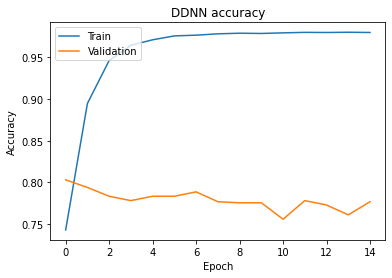
\includegraphics[width=0.8\hsize]{figuras/dnn_complex.png}
\caption{Acurácia da rede neural densa complexa.}
\label{dnn:complex}
\end{figure}

Afim de reduzir o \textit{overfitting} e obter resultados melhores, simplificamos o modelo da rede. Em seguida, utilizamos um modelo consideravelmente mais simples de apenas 3 camadas com 5357, 20 e 1 nós. Este modelo alcançou 83,0\% de acurácia de treino e 82,1\% de validação na segunda época. Apesar de obtermos resultados melhores, o \textit{overfitting} foi tão significativo quanto na rede complexa.

Todas as arquiteturas foram testadas com \textit{ReLu} nas camadas ocultas e \textit{Sigmoide} na de saída. Os treinamentos foram realizados por 15 épocas, utilizando um \textit{batch} de 100 amostras por iteração e 10\% do conjunto de disponível para validação escolhidos aleatoriamente.

As curvas de aprendizados dos modelos mencionados estão ilustradas nas \textbf{Figuras \ref{dnn:complex}} e \textbf{\ref{dnn:basic}}, respectivamente.

\begin{figure}[ht]
\centering
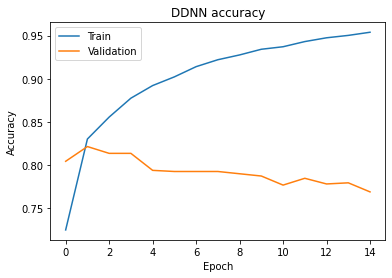
\includegraphics[width=0.8\hsize]{figuras/dnn_simple.png}
\caption{Acurácia da rede neural densa simples.}
\label{dnn:basic}
\end{figure}

\subsection{Redes Neurais Recorrentes (RNR)}

    Contrário ao esperado, todos os testes feitos com estes modelos retornaram resultados piores que os da RND. Tanto utilizando o preprocessamento básico quanto o \textit{GloVe} (\textbf{Figura \ref{rnn:glove}}), ambos os casos apresentaram \textit{overfitting} alcançando rapidamente uma acurácia de treino de quase 100\% enquanto dificilmente excederam 80\% de acurácia de validação. Os treinamentos foram realizados por 10 épocas, utilizando um \textit{batch} de 32 amostras por iteração e 10\% do conjunto de disponível para validação escolhidos aleatoriamente.
    
    A fim de melhorar os resultados, modificamos a arquitetura adicionando uma camada de \textit{max pooling} e \textit{average pooling} após a camada LSTM e concatenamos esse resultado, como proposto por Rahul Agarwal~\cite{rnn-pooling}. Mesmo com variações do modelo RNR, não conseguimos alcançar resultados melhores que os da RND, embora a adição de \textit{pooling} e o uso de \textit{GloVe} tenham ajudado a erguer os resultados.
    
    Uma hipótese que talvez justifique esta diferença entre os dois modelos é que a ordem das palavras talvez não seja tão relevante para a classificação em questão. Isso justificaria a acurácia quase perfeita no conjunto de treinamento da RNR e a baixa acurácia de validação: a adição de informação supérflua para o problema faz que que o \textit{overfitting} seja maior do que o observado na RND.

    %Observa-se, ao comparar as \textbf{Figuras \ref{rnn:basic}} e \textbf{\ref{rnn:glove}}, que o uso de \textit{word embbedings} apresentou melhorias tanto na performance quanto no \textit{overfitting}. 

%\begin{figure}[ht]
%\centering
%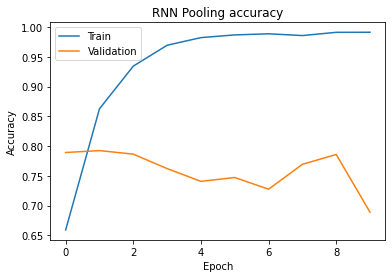
\includegraphics[width=0.8\hsize]{figuras/rnn_acc_simple.png}
%\caption{Acurácia da rede recorrente com preprocessamento básico.}
%\label{rnn:basic}
%\end{figure}

\begin{figure}[ht]
\centering
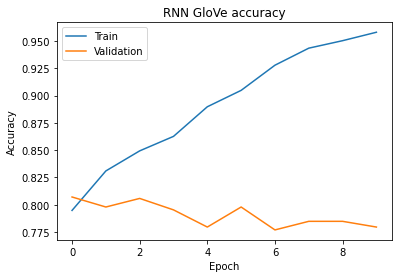
\includegraphics[width=0.8\hsize]{figuras/rnn_acc_glove.png}
\caption{Acurácia da rede recorrente com \textit{GloVe}.}
\label{rnn:glove}
\end{figure}

%\subsection{Redes Neurais Convolucionais (RNC)}

%Assim como o modelo recorrente, o modelo convolucional não gerou bons resultados quando comparado com a RNDSs. Utilizando o \textit{GloVe} como preprocessamento, criamos a seguinte arquitetura: camada de convolução $1D$, ativação \textit{ReLu}, camada de \textit{max pooling} $1D$ e por fim uma camada densa seguida da camada de ativação de saída. Dadas as condições, obtivemos os seguintes resultados: 90,4\% de acurácia de treino e 79,8\% de validação. Notou-se que o \textit{overfitting} para o modelo convolucional não foi tão significativo quanto o das RNDs e das RNRs, pois, apesar do aumento da acurácia de treino, a acurácia de validação se manteve relativamente estável.

%\begin{figure}[ht]
%\centering
%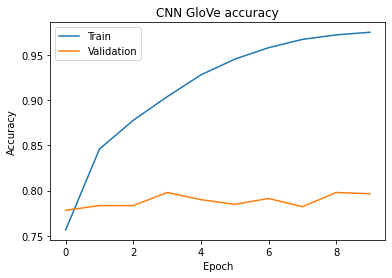
\includegraphics[width=1\hsize]{figuras/cnn.png}
%\caption{Acurácia da rede convolucional com \textit{GloVe}.}
%\label{cnn:glove}
%\end{figure}

\subsection{Redes Neurais Quasi-Recorrentes (RNQR)}

A partir do resultado decepcionante das redes recorrentes, a alternativa descrita na seção \ref{qrnn_att} foi testada, com uma arquitetura quase igual à melhor rede recorrente encontrada mas substituindo a camada BLSTM pela camada QRNN. 

A camada QRNN usou como hiperparâmetros uma janela de tamanho 3, \textit{dropout} de 20\%, regularização L2 com $\lambda = 0.001$ e restrição \textit{MaxNorm} de 10. Foi escolhido o otimizador Adam, e como função de erro a entropia cruzada binária. Na execução, foi definido um \textit{batch} de 100 amostras, e o treinamento foi feito por 15 épocas, com 10\% dos dados de treinamento separados para validação. O mesmo foi feito para a versão com \textit{self-attention}.

Os resultados obtidos, surpreendentemente, foram superiores aos das redes recorrentes testadas, passando de 81\% de acurácia de validação, com acurácia de treinamento similar. Notou-se que o \textit{overfitting} para o modelo não foi tão significativo quanto o das RNDs e das RNRs, pois, apesar do aumento da acurácia de treino, a acurácia de validação se manteve relativamente estável nas primeiras épocas, especialmente na versão com \textit{self-attention}. 

\subsection{BERT}

O último método testado foi o BERT, com a arquitetura de afinação simples descrita na seção anterior. Foi definido um \textit{batch} de 32 amostras.

Esse método se demonstrou lento para treinar com o \textit{batch} escolhido. Em média, um \textit{batch} levou 71 segundos para treinar a rede, resultando em um tempo de aproximadamente 4 horas e 15 minutos para execução de cada época. Como o \textit{Google Colaboratory} possui tempo máximo de execução, apenas 2 épocas completas puderam ser treinadas. A rede final tem 109483009 parâmetros treináveis, então faz sentido o tempo por \textit{batch}.

Mesmo com esse problema, o resultado foi muito positivo. Na segunda época foram obtidos os resultados de 83,04\% de acurácia de treinamento, e 84,12\% de acurácia de validação. Ou seja, até essa época não há \textit{overfitting}, e o aprendizado da rede parece representar o problema de modo bem melhor que os outros métodos, como esperado pela complexidade do modelo e sua característica contextual, bem importante para identificar sentimento.

\subsection{Melhor Modelo e Aplicação no Conjunto de Teste}
Para a competição, o \textit{Kaggle} disponibilizou um conjunto de teste, sem os rótulos corretos. Porém, foi descoberto que o \textit{dataset} utilizado já havia sido lançado anteriormente no mesmo \textit{website}, com todos os rótulos \cite{test}. Assim, foi possível completar o conjunto. Esse conjunto de teste com rótulos foi apenas usado para testar o melhor modelo encontrado.

O melhor modelo encontrado foi o BERT. A acurácia de treinamento, nas duas épocas treinadas, foi menor que a de vários outros, mas o resultado de validação gerado foi melhor por ao menos 2\% em comparação com qualquer outro método testado. Isso indica que o modelo representou o problema de um modo melhor que os outros, e por isso ele é escolhido para aplicação no conjunto de teste.

Após redução por remoção de pontuações e \textit{tokenização} pelo mesmo objeto \textit{FullTokenizer} usado para os dados de treinamento, obtivemos uma acurácia de 83,02\%. Verifica-se que o modelo teve boa generalização, com baixa queda de acurácia em relação ao conjunto de validação ou de treinamento. Como o resultado também é bom, podemos considerar os testes bem-sucedidos.

\section{Conclusões e Trabalho Futuro} \label{conclusion}

Dentre os experimentos feitos e modelos testados, algumas observações se destacaram. 

Quanto ao pré-processamento, lidamos com diversas técnicas, que podem gerar inúmeras combinações. Dado que esta etapa é responsável por filtrar e representar as informações textuais, se bem feita, os resultados gerados podem ser substancialmente melhores. No geral, modelos pré treinados que conseguem representar numericamente certas relações entre palavras (como o \textit{GloVe}), são a melhor escolha.

Ainda assim, a qualidade do resultado obtido por redes neurais densas, se comparado a métodos com menos pré-processamento, indica que a maior redução presente naquele método pode eliminar informações enganosas e ajudar a modelar melhor o problema. O uso de diferentes tipos de pré-processamento entre os métodos pode ser um motivo para o resultado pior dos métodos recorrentes e convolucionais.

Levando em conta a diversidade de modelos testados e o fato de que estes apresentaram resultados similares, é possível que haja uma dificuldade intrínseca ao problema que dificulta a modelagem matemática deste. Uma possibilidade é a falta de contexto, podemos ter duas frases idênticas as quais dependem de alguma imagem do tuíte para o completo entendimento.

Em relação a qualidade do BERT, a sua característica bidirecional, assim como sua construção com blocos \textit{transformer} e o fato de ser autocontido, com seu próprio processo de \textit{word embedding} e tokenização, podem ser motivos importantes para o resultado obtido. Ainda assim, este é o modelo mas lento de ser treinado por ordens de grandeza, enquanto uma simples RDN apresentou resultados rápidos com uma perda de apenas 2\% de validação, enfatizando a ideia de começar os testes através de modelos simples que podem ser facilmente implementados e retornam bons resultados.

\subsection{Trabalhos Futuros}

O melhor resultado obtido certamente não é o melhor possível, e outras modificações podem aprimorar ainda mais o resultado.

Uma melhoria a ser considerada para a metodologia seria padronizar mais adequadamente o pré-processamento entre os modelos. O uso de métodos variados nesta etapa afetou a comparação entre modelos. Outro detalhe importante, o qual não tratamos neste trabalho, foi a limpeza do \textit{dataset}: correção ou remoção de dados inválidos e \textit{outliers}. Este detalhe, se importante, pode introduzir erros no treinamento, ou resultados errados em validação ou teste.

Outros tipos de redes convolucionais podem ser testadas, como por exemplo redes CNN-SVM com camadas de sentimento pré-treinadas \cite{cnn-future}. Também daria para tentar incluir o mecanismo de atenção de outras maneiras na rede. São inúmeras as possibilidades de modificações a partir das técnicas exploradas superficialmente que podem resultar em um modelo melhor para o problema.

Visando melhorar os resultados obtidos neste trabalho, também seria interessante dar continuidade a testes com BERT e modelos concorrentes, com diferentes arquiteturas, parâmetros, etc.

O código pode ser acessado no \textit{Google Drive} através do seguinte link: \url{https://bit.ly/3a8uRUA}.

%******************************************************************************
% Referências - Definidas no arquivo Relatorio.bib

\bibliographystyle{IEEEtran}

\bibliography{Relatorio}


%******************************************************************************

\end{document}
